% This template is generated based on a beamer theme, Warsw by Dr Yufeng Lin Under MIT licence. Email Contact: e.yflin@gmail.com.
%%% Local Variables:
%%% mode: latex
%%% TeX-master: t
%%% End:

\documentclass{beamer}
\usetheme{Warsaw}
%\usetheme{Madrid}
%\usepackage{algpseudocode}
%\usepackage{algorithm}
\usepackage{bookmark}
\usepackage[timeinterval=1]{tdclock}
\usepackage{algorithm2e}
\usepackage{algorithmic}
\usepackage{float}
\usepackage[centerlast]{caption}
\usepackage{pifont}
\usepackage{xcolor}
\usepackage{mathrsfs}
\usepackage{epsfig}
\usepackage{graphicx,latexsym}
\usepackage{amssymb,amsthm,amsmath}
\usepackage{longtable,booktabs}
\usepackage{subfigure}
\usepackage{url}
\usepackage{multirow}
\usepackage{float}
\usepackage{graphicx}
%\usepackage{cite}
\usepackage{enumerate}
\usepackage{mathrsfs}
\usepackage{amssymb}
\usepackage[numbers,sort&compress]{natbib}
%\usepackage{slashbox}
\usepackage{latexsym}
\usepackage{pict2e}
\usepackage{cases}
\usepackage{stfloats}
\usepackage{caption}
\usepackage{lmodern}% http://ctan.org/pkg/lm
%\usepackage[dvips]{graphicx}
%\usepackage{array}
%\usepackage{stfloats}
%\usepackage[table]{xcolor}

%%%%%%%%%%%%%%%%%%%%%%%%%%%%%%%%%%%%%%%%%%%%
\renewcommand{\baselinestretch}{1.2}
\newcommand{\norm}[1]{\lVert#1\rVert}
\newtheorem{defi}{Definition}
\newtheorem{theo}{Theorem}
\newtheorem{assum}{Assumption}
\newtheorem{rem}{Remark}
\newtheorem{algo}{Algorithm}
\newtheorem{prob}{Problem}
\newtheorem{lem}{Lemma}
%%%%%%%%%%%%%%%%%%%%%%%%%%%%%%%%%%%%%%%%%%%
\AtBeginSection[]
{
  \begin{frame}<beamer>
    \frametitle{Outline} %for section \thesection}
    \tableofcontents[currentsection]
  \end{frame}
}
\setbeamertemplate{headline}[default]
%%%%%%%%%%%%%%%%%%%%%%%%%%%%%%%%%%%%%%%%%%%%%%%%%%%%%%%%%%%%%%%%%%%%%%%%%%%%%%%

\title[COIT11238 Networked Infrastructure Foundations]{\textbf{Week 01: Computer Network Overview}}
\subtitle{Module I: Fundamentals of Network Communication}
\author[Networking and Information Security]{COIT11238 Networked Infrastructure Foundations}
\institute[School of Engendering and Technology]{Networking and Information Security\\The College of Information and Communications Technology\\Central Queensland University, Australia}
\date{Term 1, 2023}
\logo{
\includegraphics[width=1.5cm]{CQUniversity-logo.eps}}
%%%%%%%%%%%%%%%%%%%%%%%%%%%%%%%%%%%%%%%%%%%%%%%%%%%%%%%%%%%%%%%%%%%%%%%%%%%%%%%

\begin{document}

\frame{\titlepage}

\section*{Outline}


%%%%%%%%%%%%%%%%%%%%%%%%%%%%%%%%%%%%%%%%%%%%%%%%%%%%%%%%%%%%%%%%%%%%%%%%%%%%%%
\frame{\frametitle{Acknowledgement}

The presentation slides for this unit use materials drawn from the provided resources of:\\ \bigbreak

\begin{block}{} Cengage Learning Resources (2019)\\ Tomsho, G (2019),
\textbf{Guide to Networking Essentials} (8th edn.), Cengage Learning
\end{block}

As well as other materials from online resources.
}

%%%%%%%%%%%%%%%%%%%%%%%%%%%%%%%%%%%%%%%%%%%%%%%%%%%%%%%%%%%%%%%%%%%%%%%%%%%%%
\frame{\frametitle{Objectives}

\begin{itemize}
  \item Describe a computer in a network
  \item Explain computer hardware components
  \item Introduce operating systems
  \item Discuss computer networks and Internet
  \end{itemize}

    \begin{figure}[!htp]
    \centering 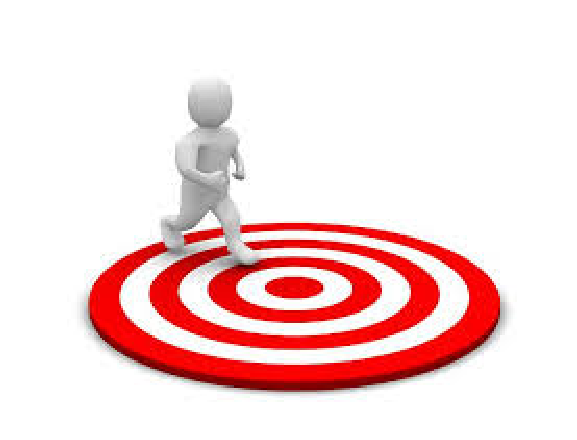
\includegraphics[width=1.5in]{Figures/Objectives.eps}
  \end{figure}

}

\section*{Outline}

\section{Networks are built from computers}
%%%%%%%%%%%%%%%%%%%%%%%%%%%%%%%%%%%%%%%%%%%%%%%%%%%%%%%%%%%%%%%%%%%%%%%%%%%%%%%%
\frame{\frametitle{An Overview of Computer Concepts}

\begin{block}{} Networks were created to facilitate communication between
computing devices, which ultimately facilitates communication between people.
\end{block}

At the heart of a communication network is the \textbf{computer}.

\begin{itemize}
  \item Most devices encountered when working with a network involve a computer
  \item Personal computers, workstations and network servers are most obvious computers running operating systems such as:\\ -- Windows, Linux, Unix, MacOS and so on.
  %\item Also including network devices: routers and switches
  %\item Nontraditional computers include: Smartphones, Amazon Echo and other
  %smart things collectively refered to as \textbf{Internet of Things (IoT)}
\end{itemize}

}

%%%%%%%%%%%%%%%%%%%%%%%%%%%%%%%%%%%%%%%%%%%%%%%%%%%%%%%%%%%%%%%%%%%%%%%%%%%%%%%%
%\frame{\frametitle{Types of Computers}
%\begin{description}
%  \item[Personal Computer] A small, single-user computer based on a
%microprocessor.
%  \item[Workstation] A workstation is like a personal computer, but it has a
%more powerful microprocessor and, in general, a higher-quality monitor.
%  \item[Minicomputer] A multi-user computer capable of supporting up to hundreds
%of users simultaneously.
%  \item[Mainframe] A powerful multi-user computer capable of supporting many
%hundreds or thousands of users simultaneously.
%  \item[Supercomputer] An extremely fast computer that can perform hundreds of
%millions of instructions per second.
%\end{description}
%
%}

%%%%%%%%%%%%%%%%%%%%%%%%%%%%%%%%%%%%%%%%%%%%%%%%%%%%%%%%%%%%%%%%%%%%%%%%%%%%%%%%
\frame{\frametitle{Personal Computer}
\begin{figure}[!htp] \centering 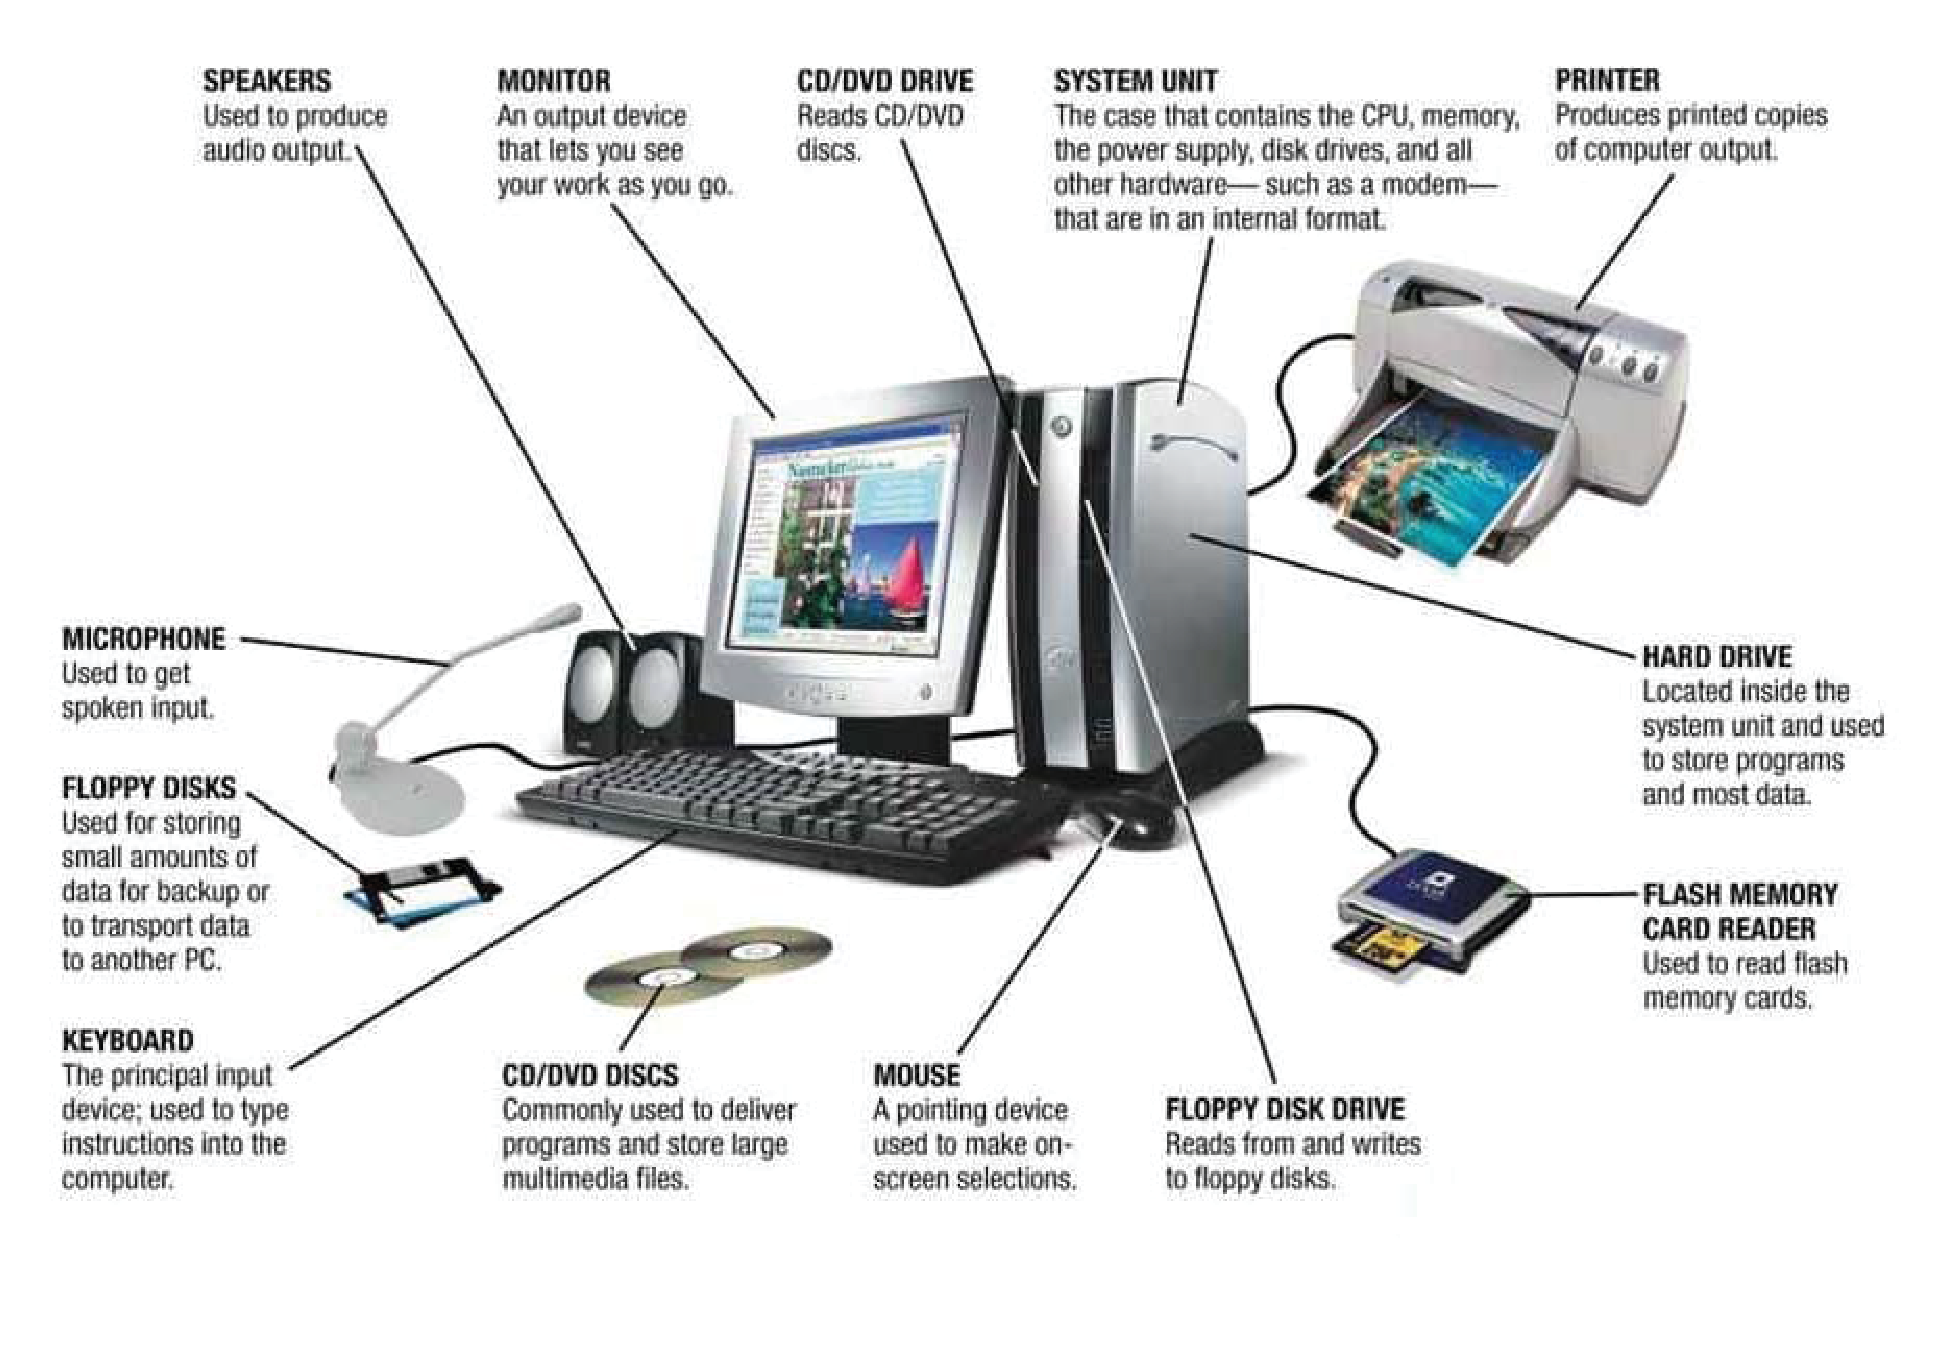
\includegraphics[width=3.2in]{Figures/PC.eps}
%\caption{} \label{fig_1}
\end{figure}

}

%%%%%%%%%%%%%%%%%%%%%%%%%%%%%%%%%%%%%%%%%%%%%%%%%%%%%%%%%%%%%%%%%%%%%%%%%%%%%%%%
\section{Computer Hardware Components}
%%%%%%%%%%%%%%%%%%%%%%%%%%%%%%%%%%%%%%%%%%%%%%%%%%%%%%%%%%%%%%%%%%%%%%%%%%%%%%%
\frame{\frametitle{Hardware Components In A Personal Computer}
\begin{figure}[!htp] \centering 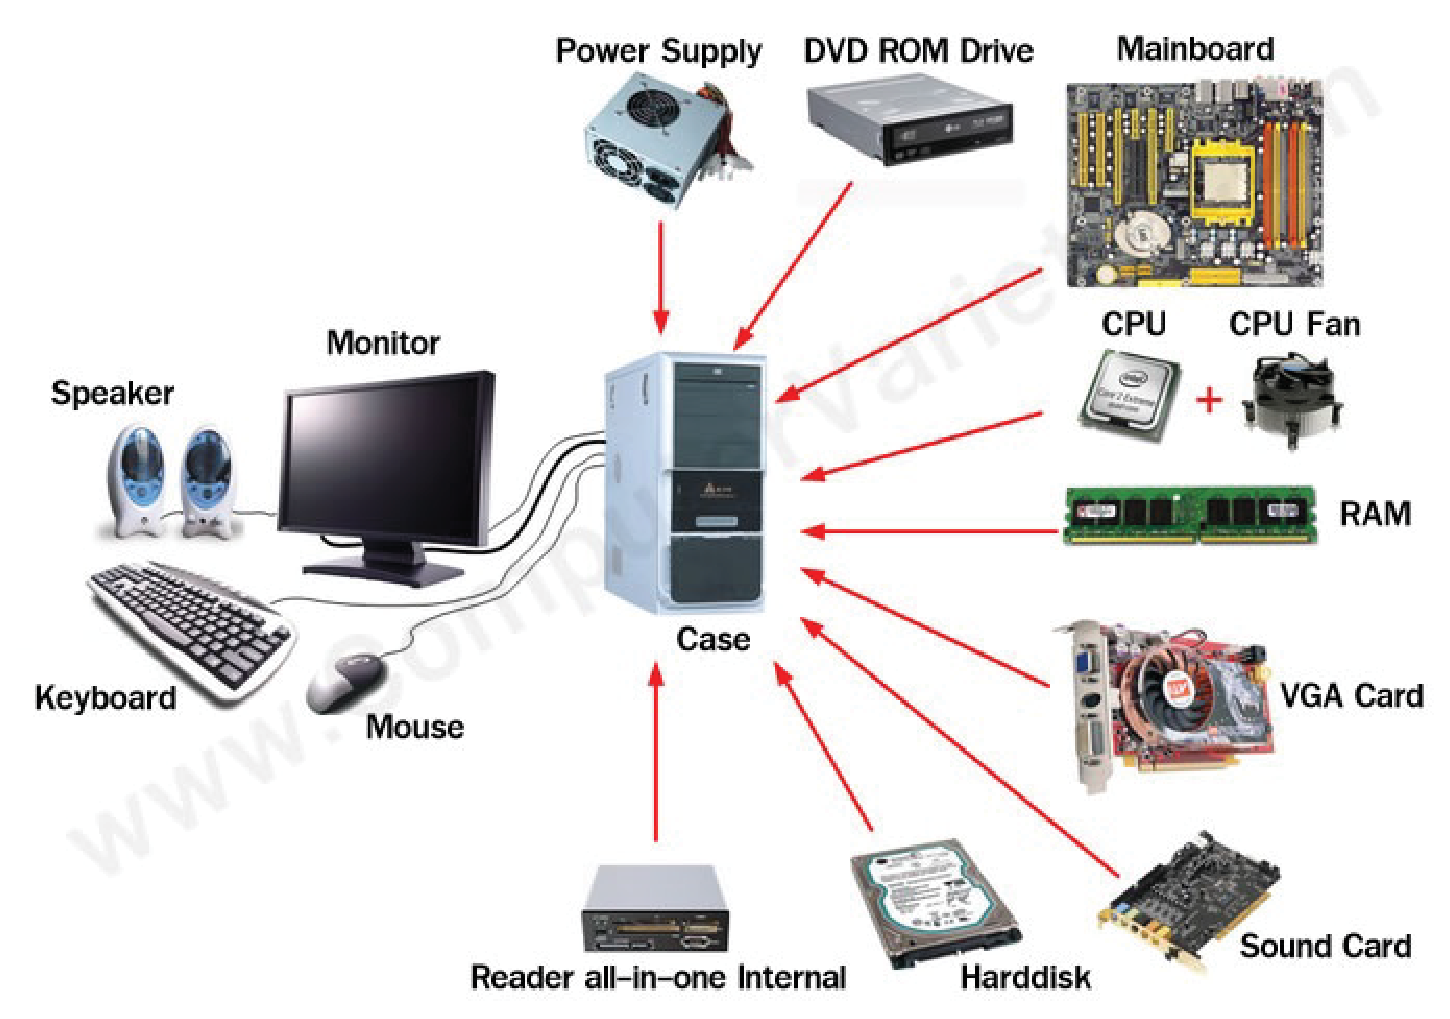
\includegraphics[width=3.2in]{Figures/aPC.eps}
%\includegraphics[width=0.01in]
%\caption{Evaluation of the window size in TCP Reno.} \label{fig_1}
\end{figure}

}

%%%%%%%%%%%%%%%%%%%%%%%%%%%%%%%%%%%%%%%%%%%%%%%%%%%%%%%%%%%%%%%%%%%%%%%%%%%%%%
\frame{\frametitle{Von Neumann Architecture}
\begin{figure}[!htp] \centering
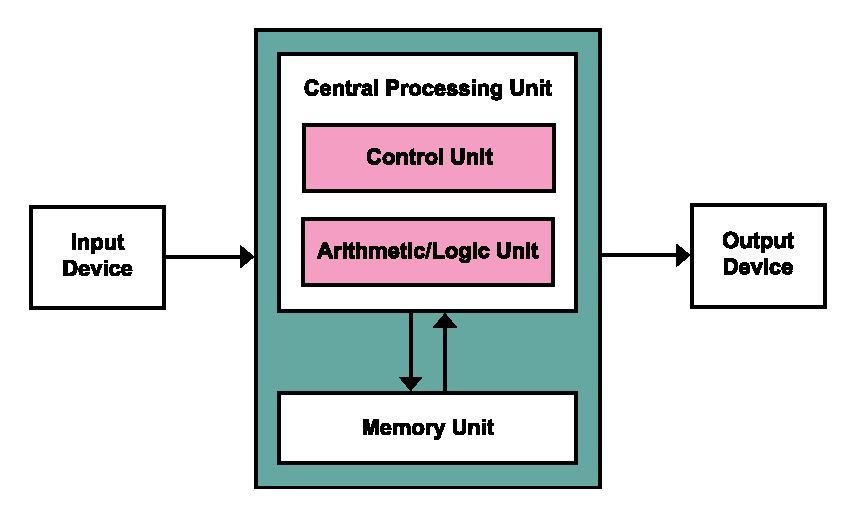
\includegraphics[width=3.2in]{Figures/Von_Neumann_Architecture.eps}
%\includegraphics[width=0.01in]
%\caption{Evaluation of the window size in TCP Reno.} \label{fig_1}
\end{figure}

}

%%%%%%%%%%%%%%%%%%%%%%%%%%%%%%%%%%%%%%%%%%%%%%%%%%%%%%%%%%%%%%%%%%%%%%%%%%%%%%
\frame{\frametitle{Basic Functions of a Computer}

\begin{itemize}
  \item A computer's functions can be broken down into three basic tasks:
  \begin{description}
    \item[\textbf{Input}] A user types the letter `A' on the keyboard, which
results in sending a code representing the letter `A' to the computer
    \item[\textbf{Processing}] The computer's CPU determines what letter was
typed by looking up the keyboard code in a table
    \item[\textbf{Output}] The CPU sends instructions to the graphics cards to
display the letter `A', which is then sent to the computer monitor
  \end{description}
\end{itemize}

}

%\frame{\frametitle{Input Components}
%
%\begin{itemize}
%  \item Includes user controlled devices such as keyboards, microphones,
%Webcams, and scanners
%  \item External interfaces, such as serial, FireWire, and USB ports can also be
%used to get input from external devices.
%  \item Input is also generated by storage devices such as hard disks and
%CDs/DVDs
%  \item Inputs to a computer can include timers that cause programs to run
%periodically
%\end{itemize}
%
%\begin{figure}[!htp]
%  \centering 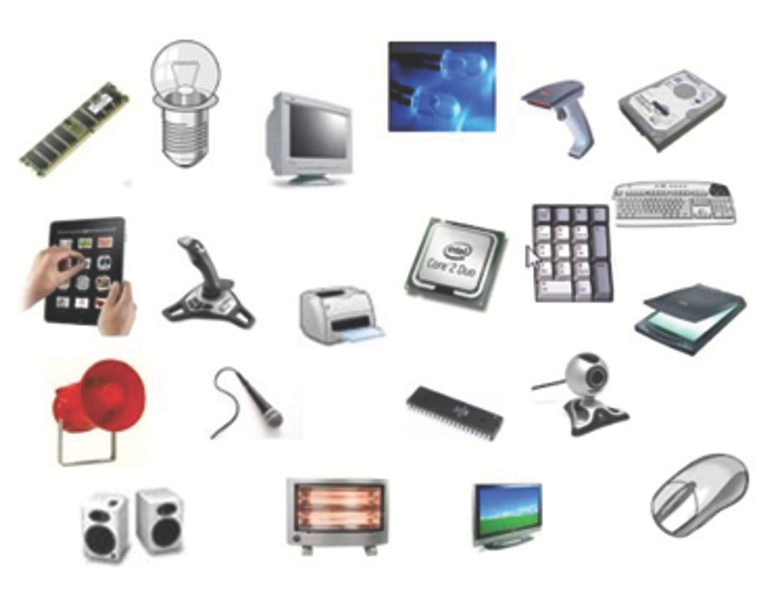
\includegraphics[width=1in]{Figures/input.eps}
%\end{figure}
%
%}
%
%\frame{\frametitle{Processing Components}
%\begin{itemize}
%  \item The CPU is a computer's main processing component
%\begin{itemize}
%  \item CPUs execute instructions from computer programs, such as word
%processors and from the computer's operating system
%\end{itemize}
%  \item Current CPUs are composed of two or more processors called
%\textbf{cores}
%      \begin{itemize}
%        \item A \textbf{multicore CPU} is like a person with two brains
%        \item Multicore CPUs enable computers to carry out multiple
%instructions/tasks simultaneously, which results in better overall performance
%      \end{itemize}
%
%    \end{itemize}
%\begin{figure}[!htp]
%  \centering 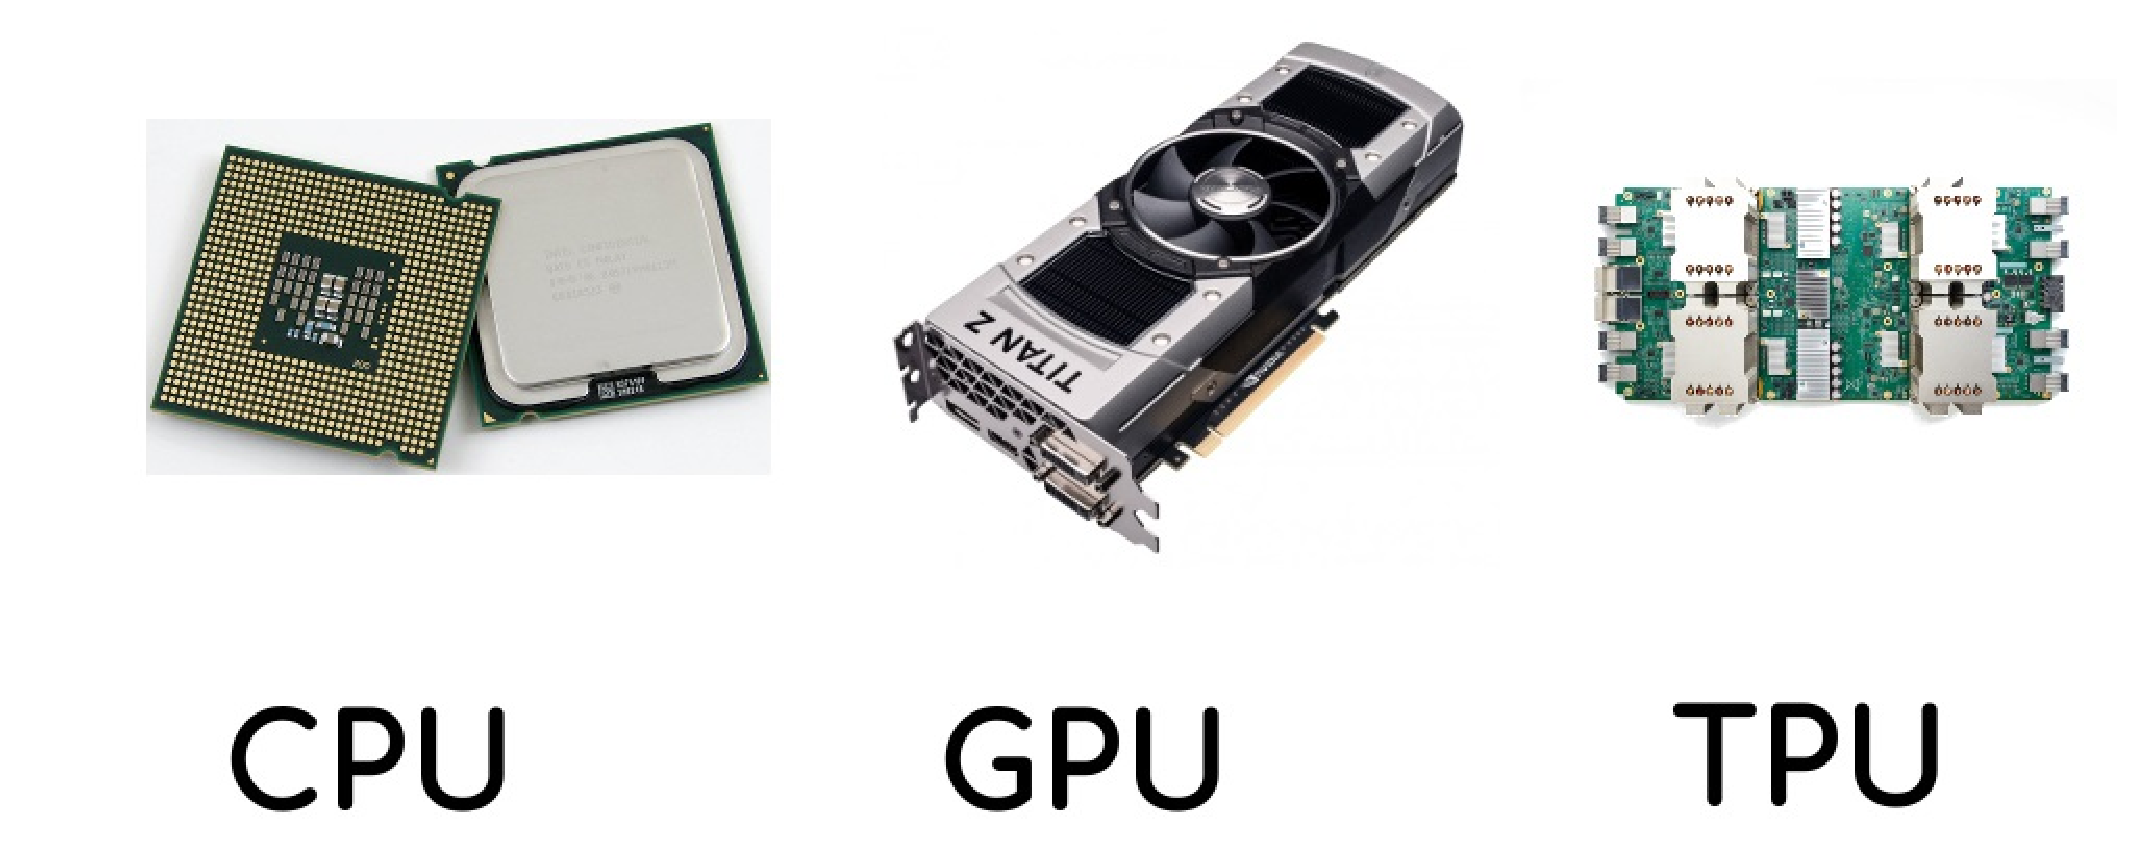
\includegraphics[width=2in]{Figures/CPU-GPU-TPU.eps}
%\end{figure}
%
%  }
%
%  \frame{\frametitle{Output Components}
%    \begin{figure}[!htp]
%  \centering 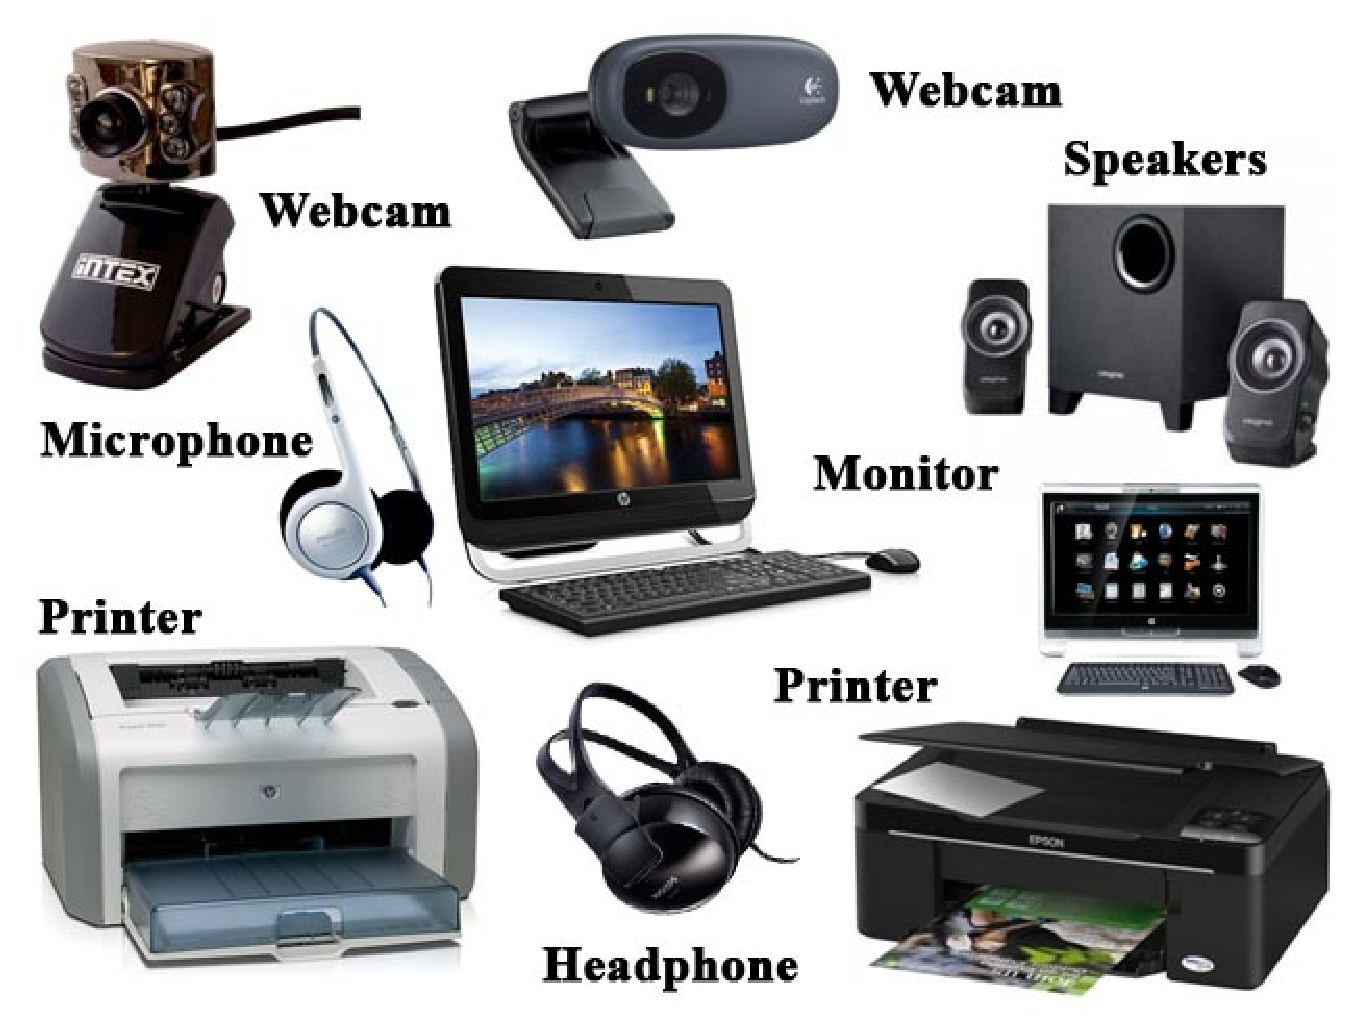
\includegraphics[width=2in]{Figures/output.eps}
%\end{figure}
%\begin{itemize}
%  \item The most obvious are monitors and printers
%  \item Also include storage devices, network cards, and sound cards
%  \item External interfaces
%\begin{itemize}
%  \item For example, a disk drive connected to a USB port allows reading files
%from the disk (input) and writing files to the \\disk (output)
%
%\end{itemize}
%\end{itemize} }

\frame{\frametitle{Storage Components}

  \begin{itemize}
  \item Short-term Storage: Random Access Memory (RAM)
    \begin{itemize}
    \item RAM is ``working storage'' because when power to the computer is
turned off, the contents in RAM are gone.
    \item The amount of RAM in a computer is crucial to the computer;s
capability to operate efficiently.
    \end{itemize}
  \item Long-term Storage
    \begin{itemize}
    \item Long-term storage, such as hard discs, CDs/DVDs Solid state
drives(SSDs), USB flash drives, maintains its data even when there's no power.
    \item The amount of storage a computer needs depends on the type and
quantity of files to be stored.
    \end{itemize}
  \end{itemize} }

\frame{\frametitle{How data is stored}
  \begin{itemize}
  \item Data on a computer is stored as binary digits(``bits'' for short)
  \item A bit holds `1' or `0' value
  \item A pulse of 5 volts of electricity can represent a bit of `1' and a pulse
of 0 volts (the absence of voltage) can represent a bit of `0'.
  \item With fiber-optic cable, a bit of `1' represented by the presence of
light and a bit of `0' by the absence of light
  \item A ``\textbf{byte}'' is a collection of 8 bits
  \end{itemize} }

\frame{\frametitle{Prefixes used for expressing bits and bytes}
\begin{table}[tp]
\caption{Prefixes used for expressing bits and bytes}
\begin{tabular}{p{3cm}p{3cm}}

  \hline
  \textbf{Prefix} & \textbf{Value} \\
  \hline
  Kilo (K) & Million ($10^6$) \\
  Giga (G) & Billion ($10^9$) \\
  Tera (T) & Trillion ($10^12$) \\
  Peta (P) & Quadrillion ($10^15$) \\
  Exa (E) & Quintillion ($10^18$) \\
  Zeta (Z) & Sextillion ($10^21$) \\
  Yotta (Y) & Septillion ($10^24$) \\
  \hline
\end{tabular}
\end{table}

}

\frame{\frametitle{Personal Computer Hardware}
  \begin{itemize}
  \item Four major PC components:
    \begin{itemize}
    \item \textbf{Motherboard}
    \item \textbf{Storage device}
    \item \textbf{RAM}
    \item \textbf{Firmware}
    \end{itemize}

  \item The Motherboard and its components
    \begin{itemize}
    \item The motherboard is a network of wires and controlling circuits that
connects all computer components
    \item Key components of a mother board are labeled in the flowing figure and
explained on the next slide following the figure
    \end{itemize}
  \end{itemize} }

\frame{\frametitle{A PC Motherboard}

\begin{figure}
  \centering
  % Requires \usepackage{graphicx}
  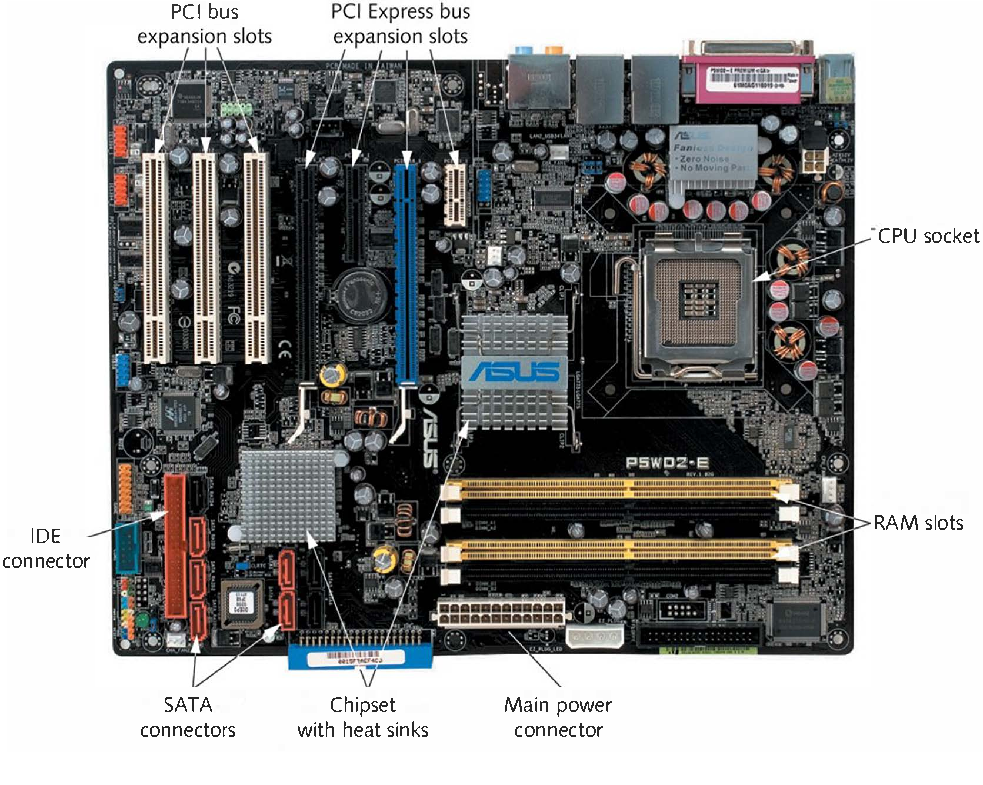
\includegraphics[width=3.2in]{Figures/Picture1_A_PC_motherboard.eps}\\
  \caption{A PC Motherboard}\label{PC_Motherboard}
\end{figure}

}
%%%%%%%%%%%%%%%%%%%%%%%%%%%%%%%%%%%%%%%%%%%%%%%%%%%%%%%%%%%%%%%%%%%%%%%%%%%%%%%
%\frame{\frametitle{Personal Computer Hardware}
%\begin{figure}
%  \centering
%  % Requires \usepackage{graphicx}
%  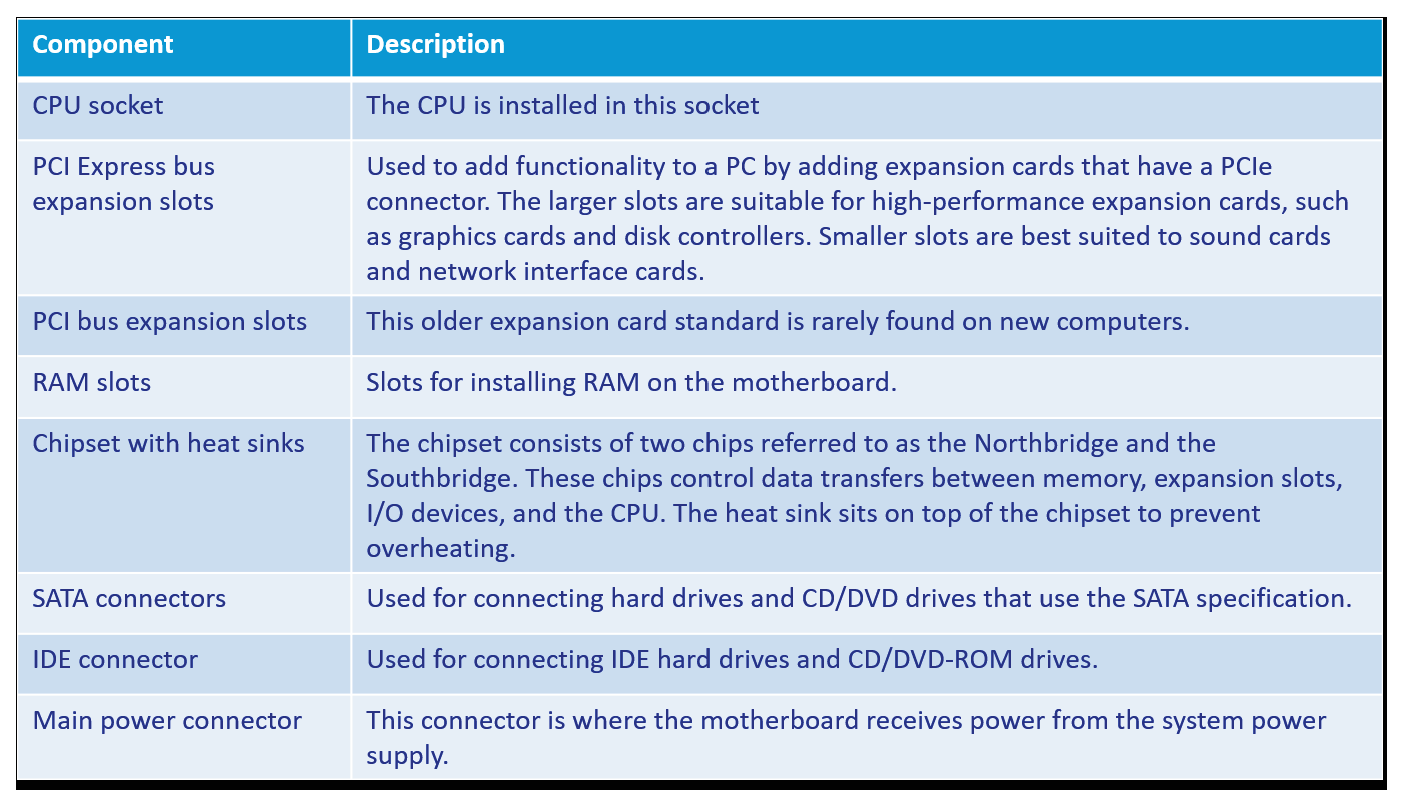
\includegraphics[width=4in]{Figures/PC_components.eps}\\
%  \caption{PC components}\label{PC_components}
%\end{figure}
%
%}
%
%%%%%%%%%%%%%%%%%%%%%%%%%%%%%%%%%%%%%%%%%%%%%%%%%%%%%%%%%%%%%%%%%%%%%%%%%%%%%%%%%
%\frame{\frametitle{Computer Bus Foundation}
%  \begin{itemize}
%  \item A \textbf{Bus} is a collection of wires carrying data from one place to
%    another no the computer.
%
%  \item All data that goes into or comes out of a computer goes through the
%    motherboard
%  \item There are buses between:
%    \begin{itemize}
%    \item CPU and RAM
%    \item CPU and disk drives
%    \item CPU and expansion slots
%    \end{itemize}
%  \end{itemize}
%}

%%%%%%%%%%%%%%%%%%%%%%%%%%%%%%%%%%%%%%%%%%%%%%%%%%%%%%%%%%%%%%%%%%%%%%%%%%%%%%%%
\frame{\frametitle{Storage Device Fundamentals}
  \begin{itemize}
  \item Hard Drive
    \begin{itemize}
    \item Hard drive is the primary long-term storage component on a computer
      \begin{itemize}
      \item Consists of magnetic disks called ``platters''
        that store data in the form of magnetic pulses
      \end{itemize}

    \item Hard disks store the documents you use as well as the applications
      that open those documents
      \begin{itemize}
      \item Also stores the OS your computer loads when it boots
      \end{itemize}
    \end{itemize}
  \item Solid State Drives
    \begin{itemize}
    \item SSDs are used in place of hard drives due to speed and reliability
    \item SSDs use flash memory
      \begin{itemize}
      \item Contains no moving parts and has faster access times
      \end{itemize}
    \item SSDs are more expensive than hard drives and are often found in mobile
      devices
      \begin{itemize}
      \item Also found in high-performance desktops and servers
      \end{itemize}
    \end{itemize}
  \end{itemize}
}

%%%%%%%%%%%%%%%%%%%%%%%%%%%%%%%%%%%%%%%%%%%%%%%%%%%%%%%%%%%%%%%%%%%%%%%%%%%%%%%%
\frame{\frametitle{RAM Fundamentals}
  \begin{itemize}
  \item RAM is the main short-term storage component on a computer
  \item Because RAM requires continuous power to store data it is referred to as
    \textbf{volatile memory}
  \item RAM has no moving parts so accessing data in RAM is much faster than
    accessing data on a hard drive
  \item In general, the more RAM your system has the faster it will run
  \end{itemize}
}

%%%%%%%%%%%%%%%%%%%%%%%%%%%%%%%%%%%%%%%%%%%%%%%%%%%%%%%%%%%%%%%%%%%%%%%%%%%%%%%%
%\frame{\frametitle{Firmware Fundamentals}
%  \begin{itemize}
%  \item Firmware is a computer program stored in nonvolatile memory such as ROM
%    or flash memory
%    \begin{itemize}
%    \item It is located on the motherboard and is executed when the computer is powered on
%    \end{itemize}
%  \item Firmware on most PCs is called the basic input/output system (\textbf{BIOS}) or
%    Unified Extensible Firmware Interface (\textbf{UEFI})
%    \begin{itemize}
%    \item Tells the CPU to perform certain tasks when power is first applied to
%      the computer
%    \item One of those instructions is to perform a power-on self test (\textbf{POST})
%    \end{itemize}
%  \item When a computer boots, the firmware program offers a chance to run the
%    Setup utility in order to configure hardware components
%    \begin{itemize}
%    \item This configuration is stored in a type of memory called complementary
%      metal oxide semiconductor (\textbf{CMOS})
%    \end{itemize}
%  \end{itemize}
%}
%%%%%%%%%%%%%%%%%%%%%%%%%%%%%%%%%%%%%%%%%%%%%%%%%%%%%%%%%%%%%%%%%%%%%%%%%%%%%%%%
\section{Operating Systems}
%%%%%%%%%%%%%%%%%%%%%%%%%%%%%%%%%%%%%%%%%%%%%%%%%%%%%%%%%%%%%%%%%%%%%%%%%%%%%%%%
\frame{\frametitle{What Is An Operating System}
  \begin{figure}[tp]
    \centering
    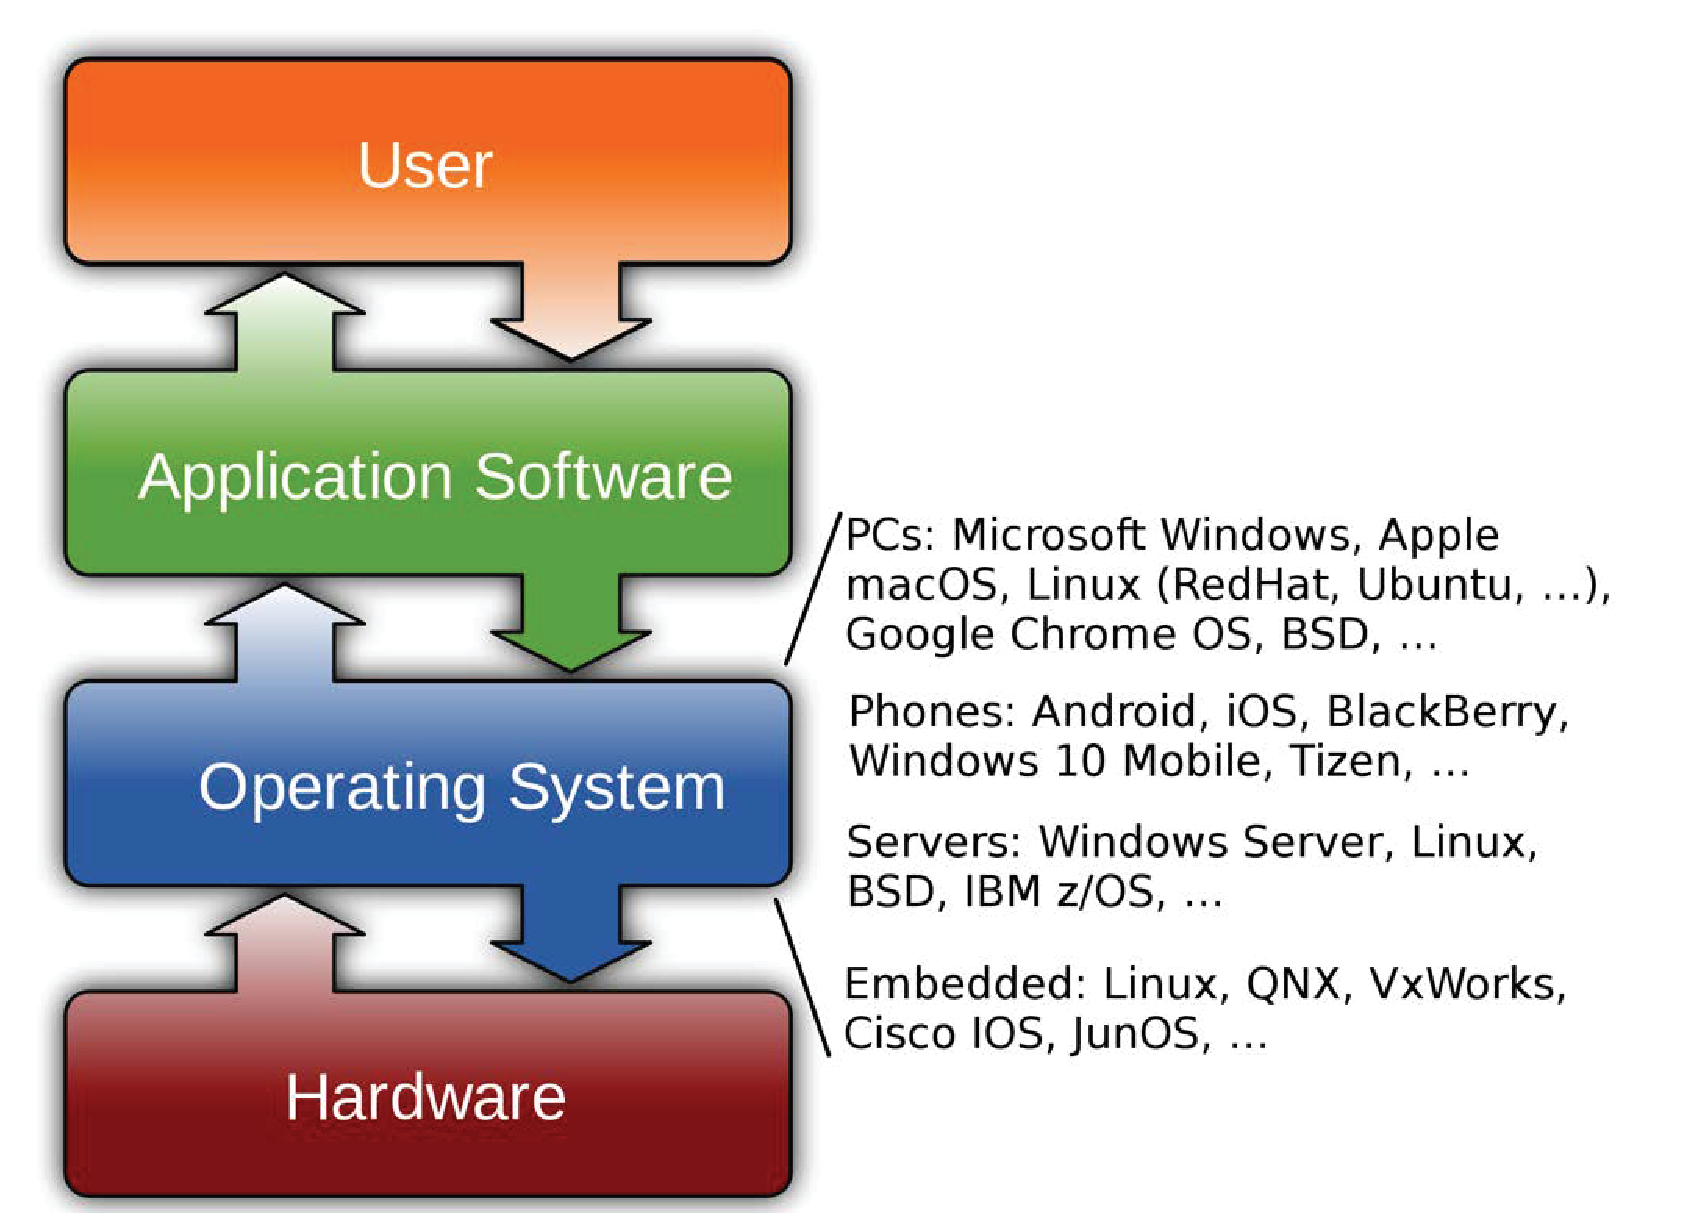
\includegraphics[width=3.3in]{Figures/System_Architecture.eps}\\
    \caption{A Simple System Architecture}
    \label{fig:system_architecture}
  \end{figure}
}

%%%%%%%%%%%%%%%%%%%%%%%%%%%%%%%%%%%%%%%%%%%%%%%%%%%%%%%%%%%%%%%%%%%%%%%%%%%%%%%%
\frame{\frametitle{Operating Systems Fundamentals}
  \begin{defi}
    An operating system (OS) is system software that manages computer hardware,
    software resources, and provides common services for computer programs.
  \end{defi}
  \begin{itemize}
  \item A computer's operating system provides a convenient interface for users
    and applications to access computer hardware components.
  \item The next few slides will expand on the following OS concepts:
    \begin{itemize}
    \item File systems
    \item Processes and services
    \item Kernel
    \end{itemize}
  \end{itemize}
}
%%%%%%%%%%%%%%%%%%%%%%%%%%%%%%%%%%%%%%%%%%%%%%%%%%%%%%%%%%%%%%%%%%%%%%%%%%%%%%%%
%\subsection{File Systems}
%%%%%%%%%%%%%%%%%%%%%%%%%%%%%%%%%%%%%%%%%%%%%%%%%%%%%%%%%%%%%%%%%%%%%%%%%%%%%%%%
\frame{\frametitle{The File System}
  \begin{itemize}
  \item A file system is the method by which an OS stores, organizes, and
    manages access to files on a storage device (such as a hard drive)
  \item File systems have the following objectives:
    \begin{itemize}
    \item Provide a convenient interface for users and applications to open and
      save files
    \item Provide an efficient method to organize space on a drive
    \item Provide a hierarchical filing method to store files
    \item Provide an indexing system for fast retrieval of files
    \item Provide secure access to files for authorized users
    \end{itemize}
  \end{itemize}
}

%%%%%%%%%%%%%%%%%%%%%%%%%%%%%%%%%%%%%%%%%%%%%%%%%%%%%%%%%%%%%%%%%%%%%%%%%%%%%%%%
\frame{\frametitle{Hierarchical Filing Method}
  \begin{itemize}
  \item Most file systems organise files in a hierarchy of folders or
    directories
  \item The top of the hierarchy is called the ``\textbf{root}'' of the file
    system
  \item Off the root of the file system can be files and folders, with folders
    containing files and additional folders (called subfolders)
  \end{itemize}
  \begin{figure}[tp]
    \centering
    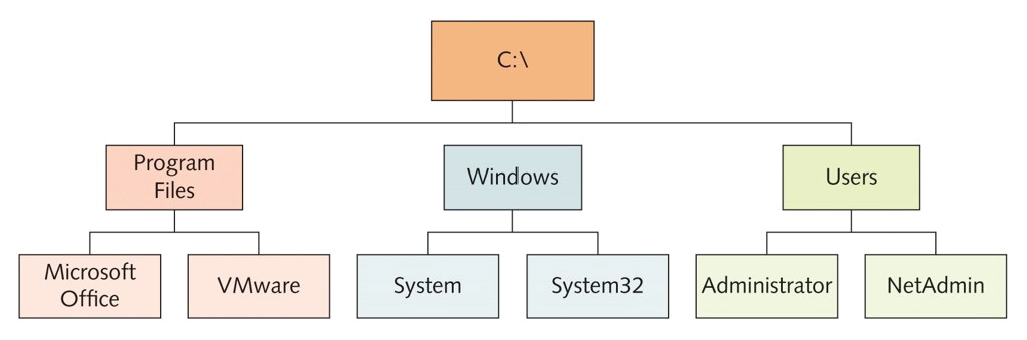
\includegraphics[width=3.3in]{Figures/A_Hierarhical_File_System.eps}\
    \caption{A hierarchical file system}
    \label{fig:file_system}
  \end{figure}
}

%%%%%%%%%%%%%%%%%%%%%%%%%%%%%%%%%%%%%%%%%%%%%%%%%%%%%%%%%%%%%%%%%%%%%%%%%%%%%%%%
\frame{\frametitle{Processes and Services}
  \begin{itemize}
  \item A \textbf{process} is a program that is loaded into memory and run by
    the CPU
    \begin{itemize}
    \item It can be an application or a program that communicates with and
      provides services to other processes (called a \textbf{service} in Windows
      and a \textbf{daemon} in Linux)
    \end{itemize}
  \item Network services allow your computer and applications to perform tasks
    they otherwise couldn't
    \begin{itemize}
    \item Example: When using a Web browser to access a Web server most people
      use a name rather than it's address. A name lookup is required before a
      Web browser can do it's main job. Domain Name Service (DNS) runs as a
      process to provide the name lookup service.
    \end{itemize}

  \end{itemize}
}

%%%%%%%%%%%%%%%%%%%%%%%%%%%%%%%%%%%%%%%%%%%%%%%%%%%%%%%%%%%%%%%%%%%%%%%%%%%%%%%%
\frame{\frametitle{Processes and Services}
\begin{itemize}
\item An OS can run many processes at the same time by using
  \textbf{multitasking}
\item A computer multitasks by using a method called \textbf{time slicing} -
  occurs when a CPU's computing cycles are divided between more than one process
  \begin{itemize}
  \item The act of changing to another process is called \textbf{context
      switching}
  \end{itemize}
  \item Two types of multitasking:
  \begin{description}
  \item[Preemptive] the OS controls which process gets access to the CPU and for
    how long
  \item[Cooperative] the OS can't stop a process, a process maintains control
    until it satisfies\\ its computing needs
  \end{description}
\end{itemize}
}

%%%%%%%%%%%%%%%%%%%%%%%%%%%%%%%%%%%%%%%%%%%%%%%%%%%%%%%%%%%%%%%%%%%%%%%%%%%%%%%%
\frame{\frametitle{Processes and Services}
\begin{itemize}
\item Many applications are now designed so that different parts can be
  scheduled to run separately
\item Each part that can be scheduled to run is called a \textbf{thread} (the
  smallest unit of software scheduled)
\item A \textbf{multithreaded application} has two or more threads that can be
  scheduled separately for execution by the CPU
\item \textbf{Multiprocessing} allows performing multiple tasks or threads
  simultaneously, each by a different CPU or CPU core

 \end{itemize}
}

\frame{\frametitle{The Kernel}
\begin{itemize}
  \item The kernel performs the following tasks:
  \begin{itemize}
  \item Schedules process to run, making sure high-priority processes are taken
    care of first
  \item Manages memory to ensure that two applications don't attempt to use
    the same memory space
    \item Makes sure I/O devices are accessed by only one process at a time
  \end{itemize}
  \item OSs are designed in layers
  \begin{itemize}
    \item The kernel is usually shown as the layer just above the hardware
  \end{itemize}
\end{itemize}
}
%%%%%%%%%%%%%%%%%%%%%%%%%%%%%%%%%%%%%%%%%%%%%%%%%%%%%%%%%%%%%%%%%%%%%%%%%%%%%%%%
\frame{\frametitle{The Windows OS Structure}
\begin{figure}
  \centering
  % Requires \usepackage{graphicx}
  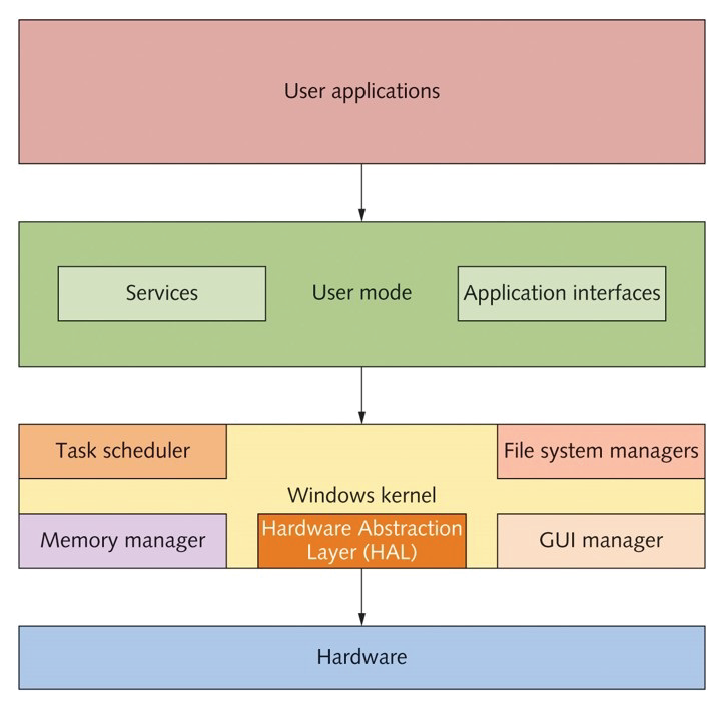
\includegraphics[width=2.5in]{Figures/The_Windows_OS_Structure.eps}\\
  %\caption{}\label{}
\end{figure}
}
%%%%%%%%%%%%%%%%%%%%%%%%%%%%%%%%%%%%%%%%%%%%%%%%%%%%%%%%%%%%%%%%%%%%%%%%%%%%%%%%
\frame{\frametitle{Client and Server Operating System Overview}
\begin{itemize}
\item Client OSs now include many features that were once only found on a server
  OS
\item The determining factor of whether you need a server OS or a client OS is
  the role the computer will play in your network
\item Client OSs usually come with client software, such as Web browsers, DNS
  and DHCP clients, and file-sharing clients
\item Most server OSs include client software but have server components, such
  as Web servers, DNS and DHCP servers, and file-sharing servers
\end{itemize}
}
%%%%%%%%%%%%%%%%%%%%%%%%%%%%%%%%%%%%%%%%%%%%%%%%%%%%%%%%%%%%%%%%%%%%%%%%%%%%%%%%
%\frame{\frametitle{Computer Boot Procedure}
%  To take a computer from a
%  powered-off state to running an OS, the following steps must take place:
%\begin{enumerate}
%  \item Power is applied to the motherboard
%  \item The CPU starts
%  \item The CPU carries out the BIOS startup routines, including the POST
%  \item Boot devices, as specified in the BIOS configuration, are searched for
%    an OS
%  \item The OS is loaded into RAM
%  \item OS services are started
%\end{enumerate}
%}
%%%%%%%%%%%%%%%%%%%%%%%%%%%%%%%%%%%%%%%%%%%%%%%%%%%%%%%%%%%%%%%%%%%%%%%%%%%%%%%%
\section{Computer Networks and the Internet}
%%%%%%%%%%%%%%%%%%%%%%%%%%%%%%%%%%%%%%%%%%%%%%%%%%%%%%%%%%%%%%%%%%%%%%%%%%%%%%%%
\frame{\frametitle{Computer Networks and the Internet}

A computer network consists of two or more computers connected by some kind of transmission medium, such as cables and/or air waves.


\begin{defi}{
\textbf{Internet}: collection of computer networks connected together using routers, where hosts and routers communicate using the Internet Protocol.
}
\end{defi}

Next week introduces computer networks, but for now let's look at some examples \ldots
}

%%%%%%%%%%%%%%%%%%%%%%%%%%%%%%%%%%%%%%%%%%%%%%%%%%%%%%%%%%%%%%%%%%%%%%%%%%%%%%%%
\frame{\frametitle{Example of A Home Network}
\begin{figure}
  \centering
  % Requires \usepackage{graphicx}
  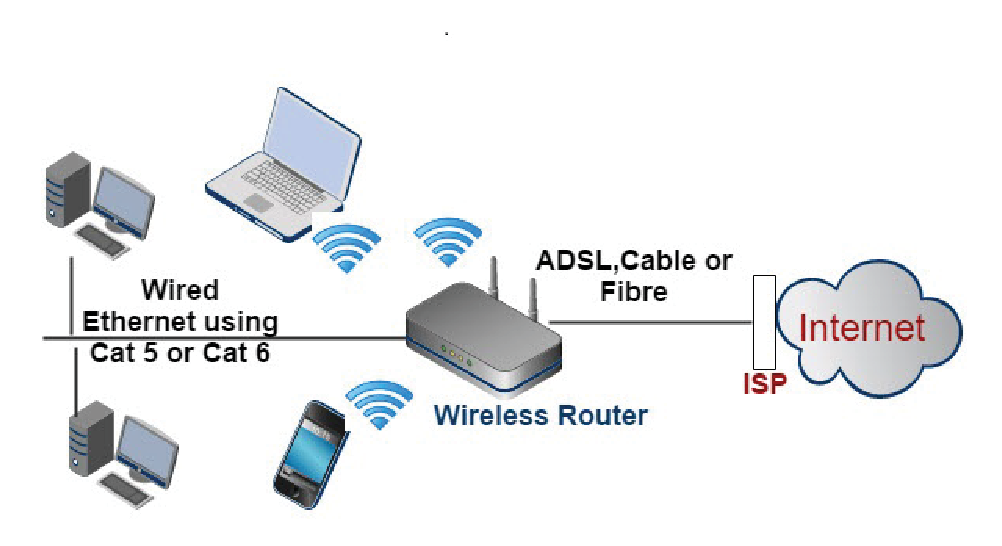
\includegraphics[width=3.5in]{Figures/home_networking_diagram.eps}\\
  \caption{An example of home networking}\label{home_networking}
\end{figure}

}
%%%%%%%%%%%%%%%%%%%%%%%%%%%%%%%%%%%%%%%%%%%%%%%%%%%%%%%%%%%%%%%%%%%%%%%%%%%%%%%%
\frame{\frametitle{Example of A University Campus Network}
\begin{figure}
  \centering
  % Requires \usepackage{graphicx}
  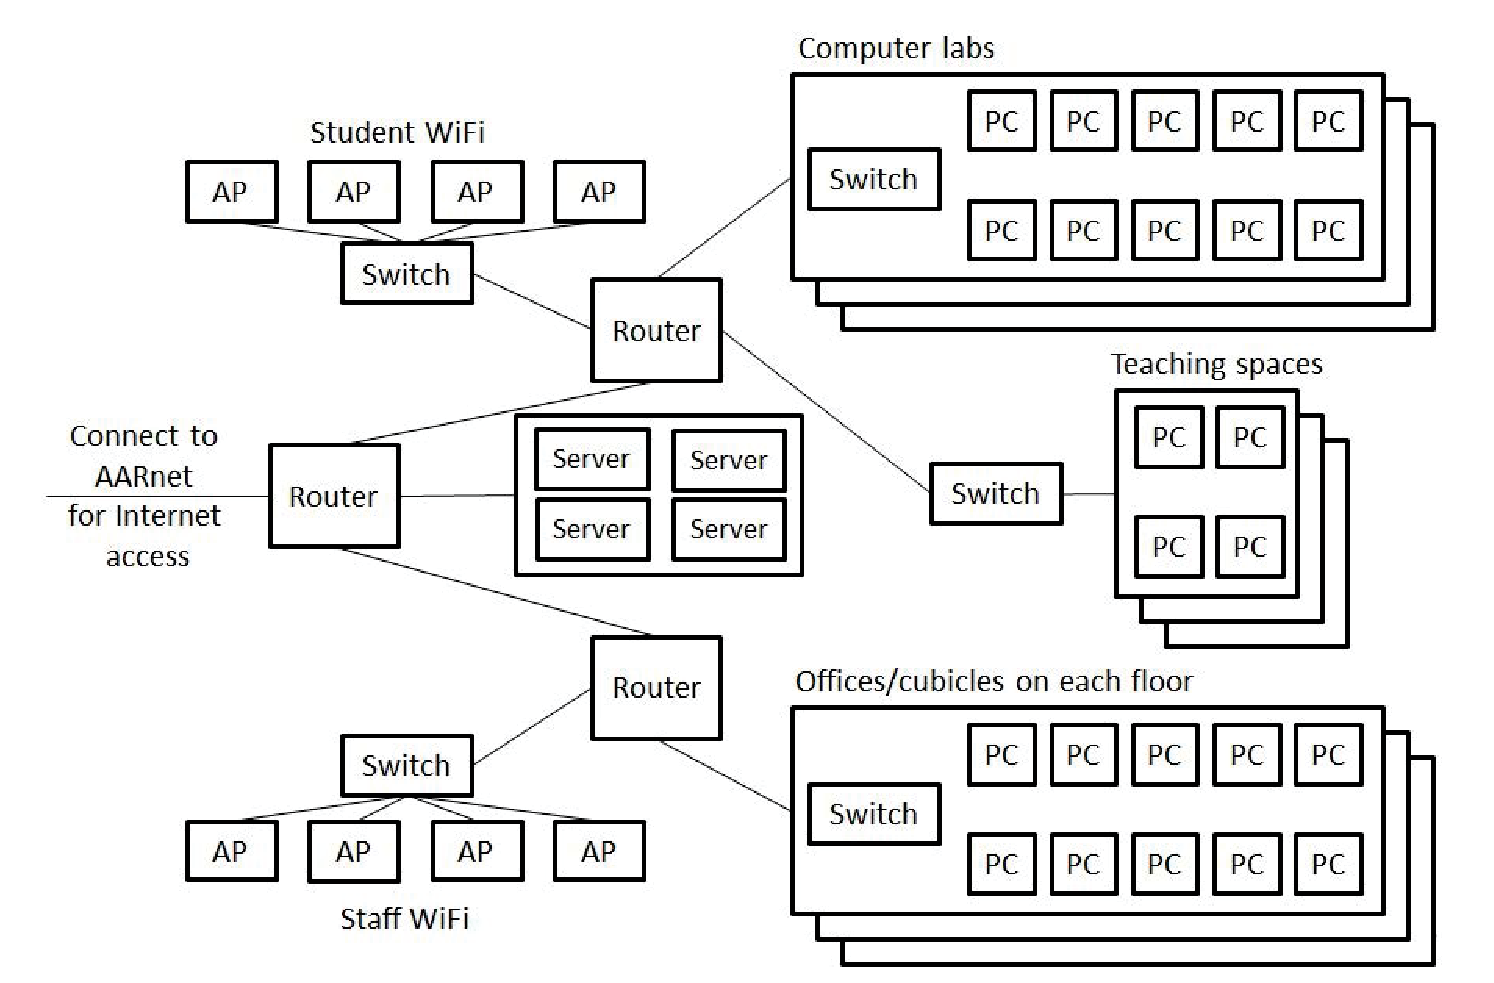
\includegraphics[width=4in]{Figures/university_campus_network.eps}\\
  \caption{An example of university campus networking}\label{campus_networking}
\end{figure}

}
%%%%%%%%%%%%%%%%%%%%%%%%%%%%%%%%%%%%%%%%%%%%%%%%%%%%%%%%%%%%%%%%%%%%%%%%%%%%%%%%
\frame{\frametitle{AARNet}

\begin{itemize}
  \item \textbf{AARNet} is the Internet Service Provider for universities in Australia
  \item Following two slides show maps of AARNet network in 2018
  \begin{description}
    \item[-] National
    \item[-] International
  \end{description}
  \item Both image are copyright AARNet:\\
  \textcolor[rgb]{0.00,0.00,1.00}{https://www.aarnet.edu.au/network-and-services/the-network}
\end{itemize}

}

\frame{
\begin{figure}
  \centering
  % Requires \usepackage{graphicx}
  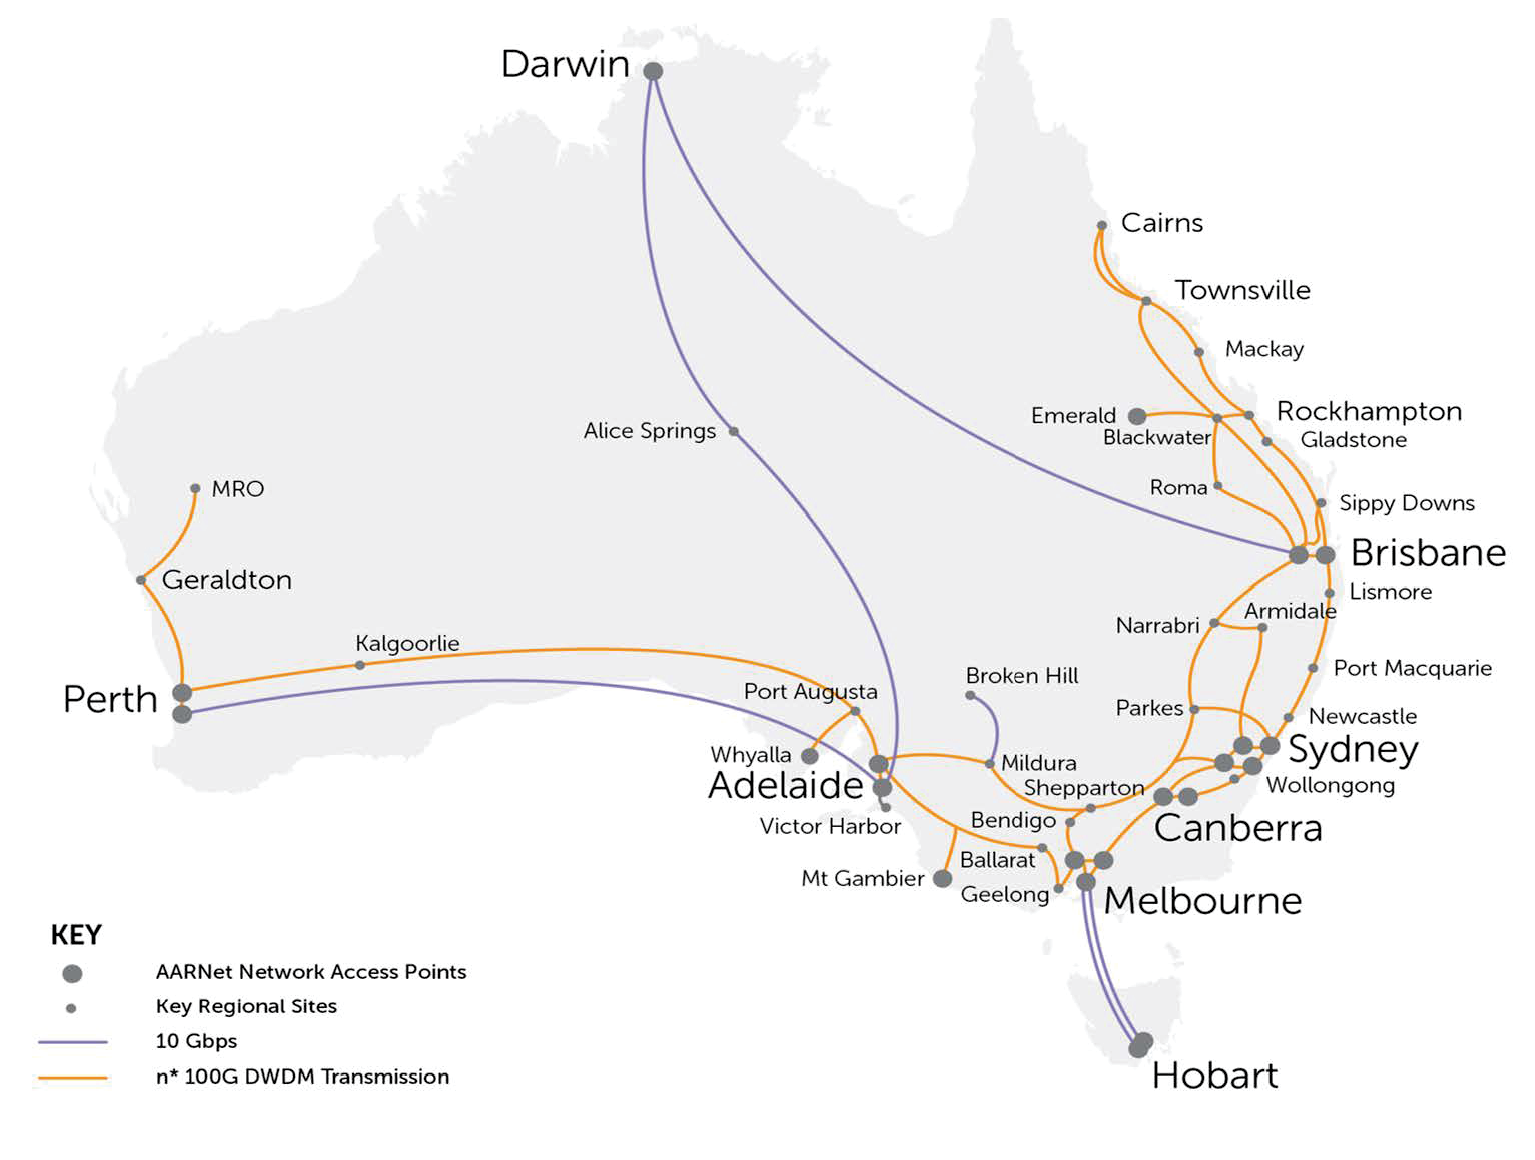
\includegraphics[width=4in]{Figures/aarnet_1.eps}\\
\end{figure}

}

\frame{
\begin{figure}
  \centering
  % Requires \usepackage{graphicx}
  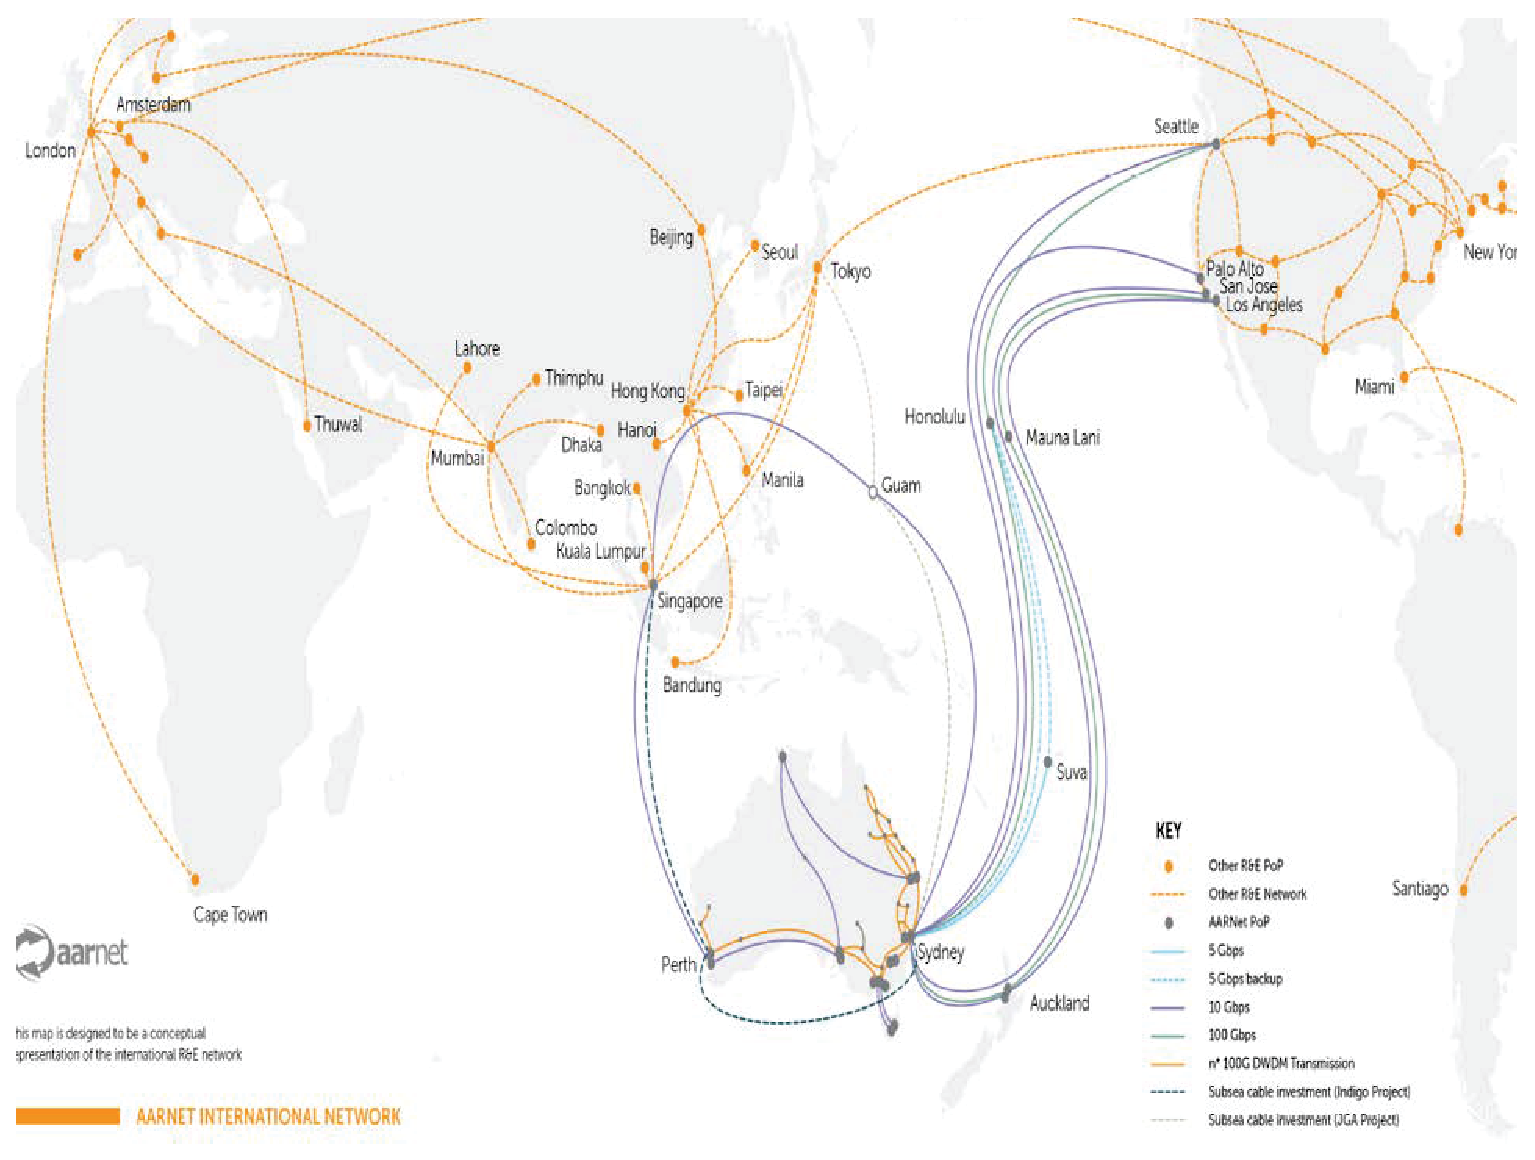
\includegraphics[width=3.6in]{Figures/aarnet_2.eps}\\
\end{figure}

}
%%%%%%%%%%%%%%%%%%%%%%%%%%%%%%%%%%%%%%%%%%%%%%%%%%%%%%%%%%%%%%%%%%%%%%%%%%%%%%%%
\frame{\frametitle{The Internet}
\begin{itemize}
  \item Visit the TeleGeography Global Internet Map
  \item \textcolor[rgb]{0.00,0.07,1.00}{https://global-internet-map-2018.telegeography.com/}\\
  -- Shows major links between countries\\
  -- Also their Submarine Cable Map:\\
     \textcolor[rgb]{0.00,0.07,1.00}{https://www.submarinecablemap.com/}
\end{itemize}

}



%%%%%%%%%%%%%%%%%%%%%%%%%%%%%%%%%%%%%%%%%%%%%%%%%%%%%%%%%%%%%%%%%%%%%%%%%%%%%%%%
%\frame{\frametitle{The Internet of Things}
%\begin{definition} \textbf{The Internet of Things (IoT)} is a concept in which
%the virtual world of Information technology integrates with the real world of
%things through network connectivity (Uckelmann, Harrison \& Michahelles, 2011).
%\end{definition}
%\begin{figure}[!htp] \centering 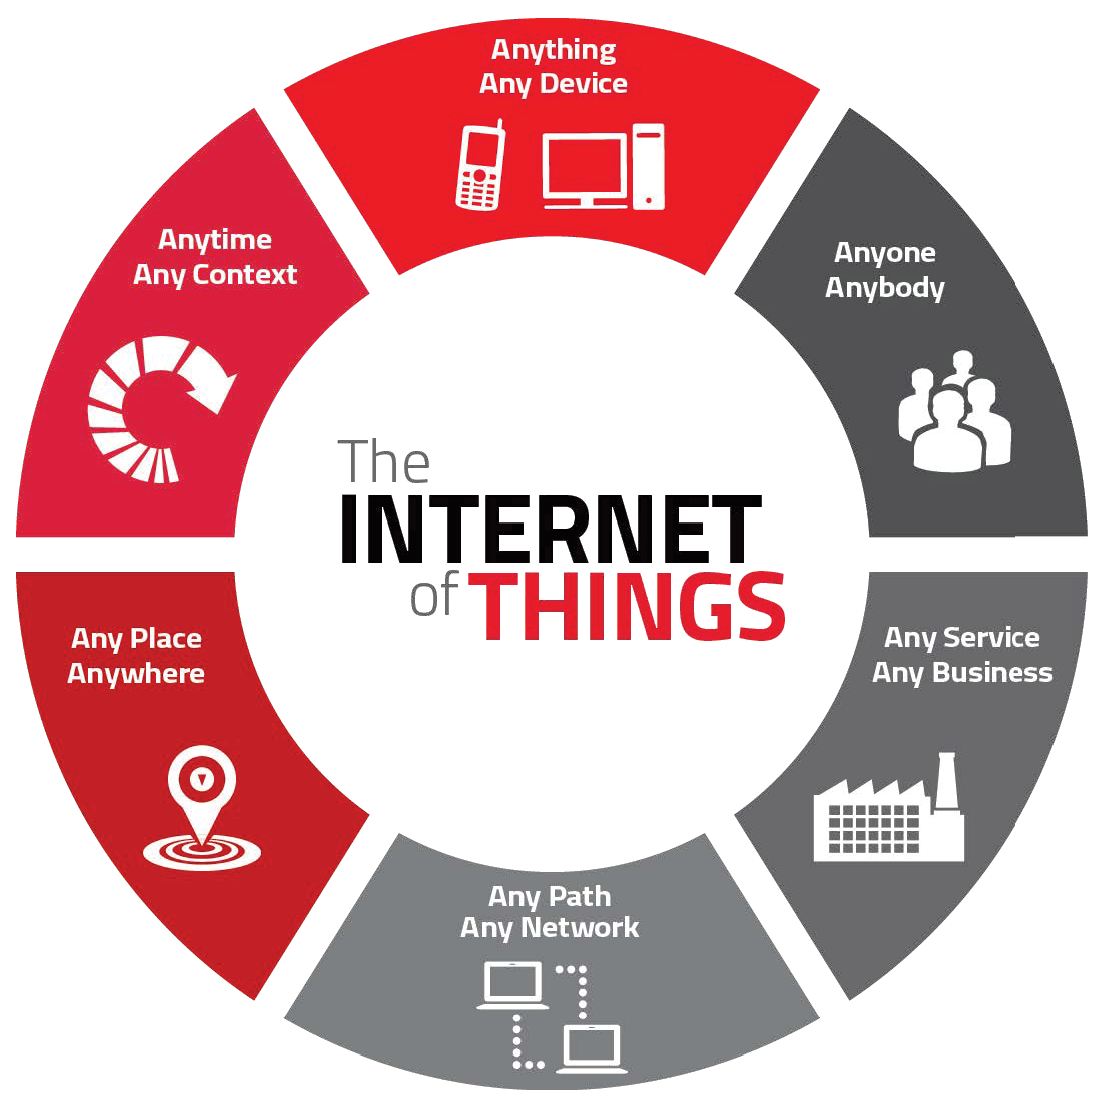
\includegraphics[width=1.75in]{IoT-1.eps}
%%\includegraphics[width=0.01in]
%%\caption{Evaluation of the window size in TCP Reno.} \label{fig_1}
%\end{figure}
%% \textbf{Advantages:}\\ %Flexible architectures, enabling remote execution,
%% easy diagnosis and maintenance \\ %...
%}

\frame{
\begin{figure}
  \centering
  % Requires \usepackage{graphicx}
  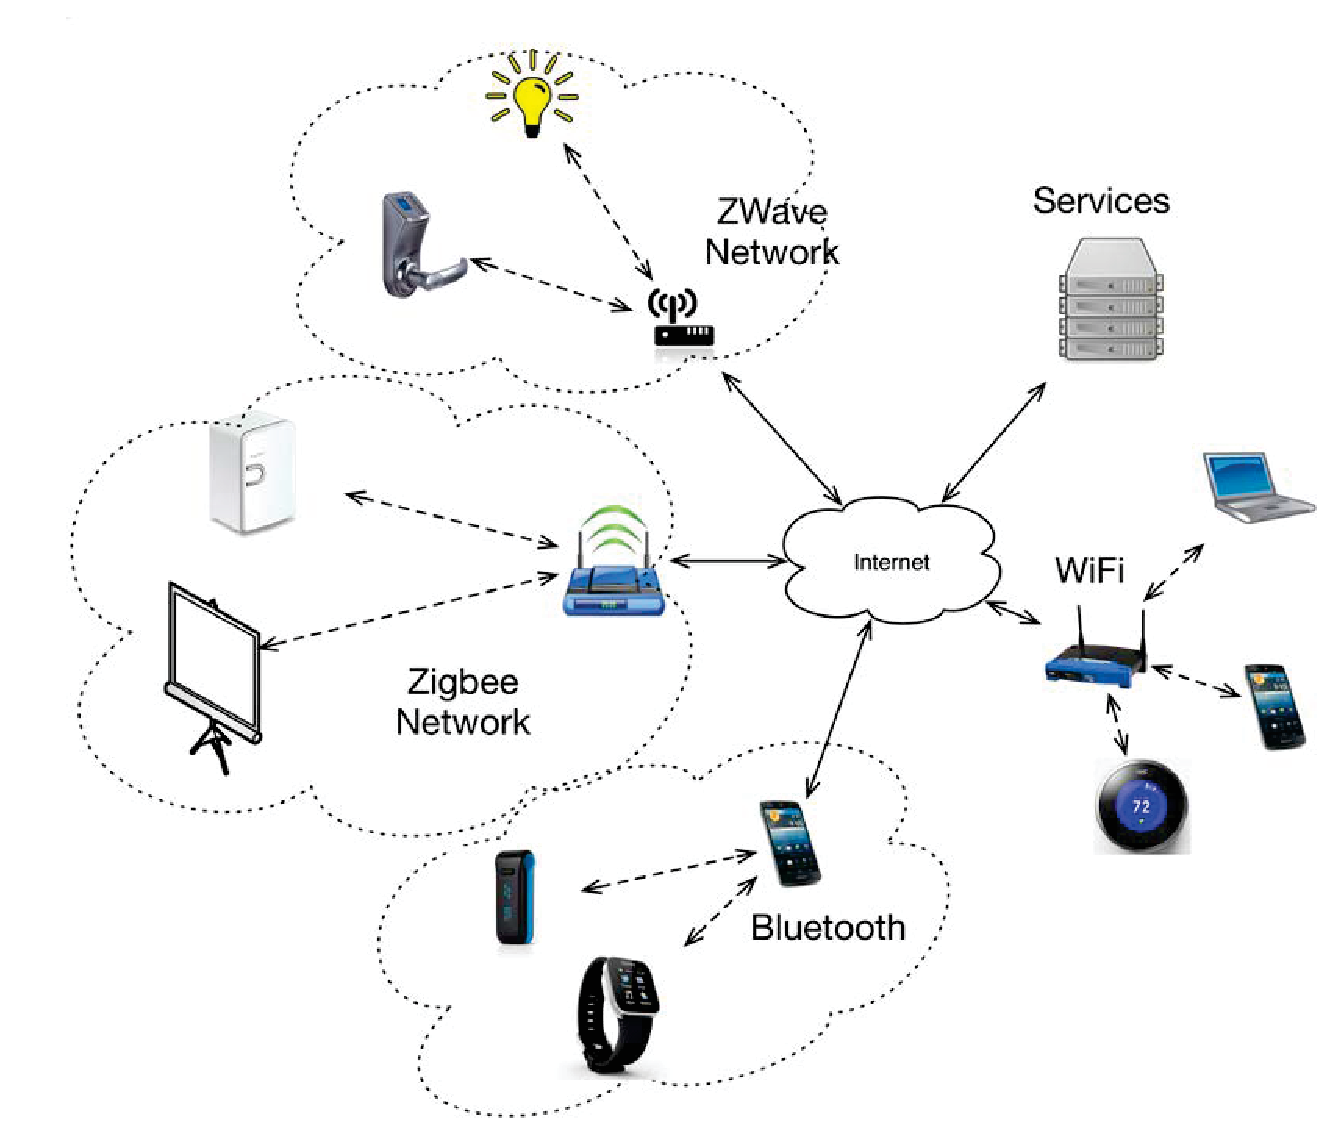
\includegraphics[width=3.5in]{Figures/IoT_network_architecture.eps}\\
\end{figure}

}

%%%%%%%%%%%%%%%%%%%%%%%%%%%%%%%%%%%%%%%%%%%%%%%%%%%%%%%%%%%%%%%%%%%%%%%%%%%%%%%%
\frame{\frametitle{Components of A Computer Network}
\begin{description}
  \item[\textbf{Computers}]PCs, laptops, phones, servers,\ldots
  \item[\textbf{Network devices}]Repeaters, modems, switches, routers, access points, \ldots
  \item[\textbf{Network media}]Copper, coax, fibre, WiFi, satellite,
  \item[\textbf{Addressing}]MAC, IP, domains, \ldots
  \item[\textbf{Protocols}]IP, TCP, HTTP, DNS, SIP, \ldots
  \item[\textbf{Software}]browsers, game servers, email clients, chat apps, network OS, \ldots
\end{description}

}

%%%%%%%%%%%%%%%%%%%%%%%%%%%%%%%%%%%%%%%%%%%%%%%%%%%%%%%%%%%%%%%%%%%%%%%%%%%%%%%%
\section{Summary}
\frame{\frametitle{Summary}
\begin{itemize}
  \item Computers in a network\\
  -- PCs, servers and embedded devices
  \item Computer hardware components\\
  -- Input, processing and output\\
  -- Motherboard, hard drive and RAM
  \item Basic features of operating systems\\
  -- Architecture, kernel and file systems\\
  -- Processes and services\\
  %-- Computer boot procedure
  \item Computer networks and Internet
  -- Examples for computer networks\\
  -- AARNet and Internet\\
%  -- IoT networks
\end{itemize}
}

\end{document}


%%% Local Variables:
%%% mode: latex
%%% TeX-master: t
%%% End:
